%!TEX root = main.tex
% revision is done
\Chapter{Введение}

\section{Парадигмы программирования}%
Когда-то, не~очень давно, работа программиста называлась «кодированием», а~программа~--- «машинным кодом». В~самих этих названиях есть что-то от~шпионских игр и~шифровки. Программисты переводили метод решения прикладных задач на~язык алгоритмов, понятный человеку, а~алгоритмы~--- в~последовательность инструкций, понятных машине. Таким образом, программа воспринималась, как текст, предназначенный для машины, а~не для человека. Для того, чтобы человек мог разобраться в~этих инструкциях, для их отладки или модификации, разрабатывались те или иные \emph{парадигмы программирования}~--- стилистические и~методологические концепции, позволяющие приблизить процесс написания и~чтения программы к~человеческому восприятию и~к предметной области решаемых программистом задач.

Разделяют две противоположные парадигмы программирования: \index{парадигма программирования!императивная}\emph{императивную} и~\index{парадигма программирования!декларативная}\emph{декларативную}. Само слово «программа» подразумевает некоторую последовательность действий, предписанную для выполнения задачи. В~этом и~проявляется императивный подход. В~нём программой является последовательность инструкций, а~вычислительным процессом~--- последовательность состояний вычислительной среды. При~декларативном подходе программа превращается в~совокупность набора определений, описывающих условие решаемой задачи, и~набора соотношений, показывающих, в~чём состоит её решение.

\index{парадигма программирования!функциональная}\emph{Функциональное программирование} (ФП)~--- это одна из~парадигм декларативного программирования. В~ней описание процесса решения задачи сводится к~определению набора функций, а~постановку задачи определяют аргументы, передаваемые этим \mbox{функциям}.

В математике \index{функция}\emph{функция}~--- это отображение из~области определения в~область значений. Когда мы говорим о~функции $f(x)$, мы одновременно подразумеваем и~процедуру отображения и~результат этого отображения: в~определённом смысле, мы в~праве смешивать эти два понятия. Такой подход к~функциям оказался пригодным и~очень продуктивным для программирования. Когда мы представляем программу, как набор функций, мы можем воспринимать их, в~зависимости от~необходимости, как процессы или как результаты, то есть, как данные.

Перечислим основные принципы ФП:

\begin{enumerate}
 \item Программирование не~опирается на~хранение состояния вычислительной среды. Вместо этого вычисляются результаты чистых функций от~исходных данных и~результатов других функций.

 \item Использование функций, как \emph{объектов первого класса}. Это значит, что функции можно использовать как данные: создавать их во~время выполнения программы, передавать их в~качестве аргументов другим функциям и возвращать в качестве результатов.

 \item Из~предыдущего вытекает возможность писать и~использовать функции высших порядков и~функционалы~--- функции, аргументами и~значениями которых являются другие функции.

 \item Использование \emph{чистых функций}~--- функций не~имеющих побочных эффектов, зависящих только от~своих аргументов и~только возвращающих свой результат.

 \item Применение \emph{рекурсии}, как основного способа описания циклических процессов.

 \item \emph{Интенсивные} и~\emph{ленивые} \emph{вычисления}, различающиеся порядком, в~котором обрабатываются аргументы функций.

\end{enumerate}

Самое же главное --- разработанная в~математике строгая теория функций применима и~к функциональным программам. Из~перечисленных нами особенностей вытекают следующие достоинства~ФП:

\begin{enumerate}
 \item Возможность строгого доказательства корректности программы и, как следствие, повышение надёжности кода.

 \item Возможность существенной оптимизации программы при~компиляции.

 \item Высокая степень абстракции и~связанные с~этим удобочитаемость, расширяемость и~переносимость программ.

 \item Использование чистых функций существенно повышает модульность программ и~упрощает организацию параллельных вычислений.
\end{enumerate}

При изучении данного курса следует помнить, что достоинства функционального программирования не~определяются достоинствами того или иного языка программирования, \Lang{Scheme} или \Lang{Haskell}, например. Они относятся к~функциональному подходу в~целом, как к~модели вычислений и~модели построения программ и~структур данных. Эта модель возникла раньше модели Тьюринга и~частично легла в~её основу. Если сначала функциональное программирование носило, преимущественно, теоретический характер, как важный инструмент теории вычислений и~алгоритмов, а~потом долго не~выходило за~рамки специализированных функциональных языков программирования, то сейчас функциональный инструментарий включается во~многие широко используемые на~практике языки: \Lang{C\#}, \Lang{Python}, \Lang{Perl}, \Lang{JavaScript} и~т.\,д. Кроме того, и~существенно функциональные языки, такие, как \Lang{OCaml}, \Lisp, \Lang{Erlang,} \Lang{Haskell}, \Lang{F\#} давно вышли из~академической среды и~стали использоваться для решения самых разных практических и~промышленных задач.

\section[4]{Зачем изучать функциональное программирование?}%
Освоение функциональной парадигмы прививает определённый стиль программирования, имеющий универсальные достоинства~--- писать «функционально» можно практически на~любом высокоуровневом языке программирования. При~этом программы становится легче читать, отлаживать и~расширять. Меняется и~подход к~формулировке задач: она становится более строгой и~предметно-ориентированной.{\tolerance=800\par}

Кроме того, большинство современных промышленных языков программирования имеет функциональный инструментарий, и~квалифицированный специалист должен уметь использовать его в~полной мере.

Наконец, немаловажным оказывается и~субъективное восприятие той или иной парадигмы. При~императивном подходе программист является «диктатором»~--- машина, получая от~него список непреложных указаний, находится в~подчинённом положении. Процесс декларативного программирования можно воспринимать, как обучение машины человеком, как передачу знаний и~умений, зачастую, превращающееся в~совместное с~машиной исследование предметной области. Именно функциональные языки программирования используются для разработки искусственного интеллекта, экспертных систем, систем обработки символьных и~вербальных данных.

\section[2]{Язык Formica}%
Для примеров в этой книге используется язык \FLP{}\footnote{https://github.com/samsergey/formica} --- диалект языка \Scheme. В свою очередь, \Scheme является наследником замечательного языка \Lang{Scheme}.

\Lang{Scheme}~--- это \emph{язык программирования высокого уровня}, один из~двух наиболее популярных в~наши дни диалектов языка \Lisp. Язык \Lang{Scheme} был создан в~середине 1970-х годов и~с тех пор широко используется и~развивается. Он, наряду с~\Lisp-ом, используется, для написания скриптов и~сценариев, например, в~таких программах, как \Lang{AutoCAD}, \Lang{Gimp}, \Lang{Emacs} и~пр. Кроме того, эти языки используются для оптимизации трансляторов и~компиляторов, для синтаксического разбора текстов; на~них пишут серверы и~веб-приложения, экспертные системы и~системы компьютерной алгебры, а~так~же многие другие приложения. Существует множество интерпретаторов и~компиляторов \Lang{Scheme}, как свободных, так и~проприетарных.

Разработчики \Lang{Scheme} старались не~нарушить элегантность и~простоту языка, его подчёркнуто минималистскую философию. Цель создания \Lang{Scheme}~--- не~собирать воедино разные полезные конструкции и~средства, а~удалить слабости и~ограничения, вызывающие необходимость добавления в~язык новых возможностей. В~результате, язык содержит минимум примитивных конструкций и~позволяет выразить всё что угодно, путём надстройки над~ними. Девиз языков семейства \Lisp: «\Lisp~--- программируемый язык программирования». По~существу, программирование на~\Lang{Scheme}~--- это создание новых языков, заточенных под~решаемые задачи.

Язык \Lang{Scheme} и его диалекты могут быть полезны в~повседневной работе программиста, даже если он использует для работы совсем другие языки. С~их помощью можно детально разрабатывать алгоритмы, концентрируясь на~существе разрабатываемого вычислительного процесса, на~вопросах корректности и~эффективности алгоритма, не~отвлекаясь, до~поры до~времени, на~детали ввода-вывода или на~менеджмент памяти.

\Lang{Scheme} не~является чистым функциональным языком, как, например, \Lang{Haskell}, но принципы, лежащие в~его основе, дают возможность писать чисто функциональные программы. Более того, этот язык позволит нам самостоятельно разработать практически весь необходимый инструментарий для полноценного программирования в~рамках функциональной парадигмы.

\subsection{Особенности Formica}%
Перечислим основные особенности \FLP:

\begin{itemize}
  \item Упрощённый синтаксис для каррирования и частичного применения функций.
  \item Наличие подстановок, реализующих технику переписывания и сопоставления с образцом.
  \item Наличие формальных функций, служащих для отладки функциональных программ, а так же для определения абстрактных и алгебраических типов данных.
  \item Гибкая система динамической типизации, позволяющая использовать абстрактные, алгебраические и полиморфные \mbox{типы}.
  \item Большое число инструментов для функционального программирования.
  \item Встроенные средства для мемоизации функций.
  \item Инструментарий для определения и использования монад.
\end{itemize}

\section{Обозначения, принятые в~тексте}%
Приводя код на~языке \Scheme, мы будем выделять с~помощью различных шрифтов различные объекты:

\begin{itemize}[\ ]
  \item \s{cons list sin} ...~--- базовые функции; 
  \item \s{define let if} ...~--- специальные формы;
  \item \s{fold f sum} ...~--- определяемые нами функции;
  \item \lex{x y expr} ...~--- формальные аргументы функций;
  \item \s[emph={}]{1 2.3 #t "abc"} ...~--- константы;
  \item \s{; some text}~--- комментарии.
\end{itemize}

\newpage
\section[2]{Программа DrRacket}%
Программа \Lang{DrRacket}\footnote{http://racket-lang.org/.} является интегрированной средой разработки программ для диалектов языка \Lang{Scheme}. Она включает в~себя редактор, компилятор и~интерпретатор, отладчик, менеджер программных модулей и~другие инструменты. Кроме этого, в~дистрибутив входит полная документация по~языку \Racket (на английском языке) и русскоязычная документация по \Scheme, которая находится в разделе \textbf{Getting started} (меню \MenuItem{Help | Help Desk}).

Программа разработана в~рамках проекта PLT (Programming Language Teaching) и~является свободно распространяемым продуктом. Существуют реализации программы \Lang{DrRacket} для различных платформ: MS Windows, Linux, MacOS и~др. Данный курс опирается на~версию \Lang{DrRacket} 5.3.1 или повышение.

Приведём основные команды программы \Lang{DrRacket}, которые нам потребуются:

\noindent
\begin{threeparttable}
\begin{tabular}{p{0.35\textwidth}p{0.15\textwidth}>{\comment\baselineskip=9pt}p{0.4\textwidth}}\toprule
\bfseries Меню & \bfseries Клавиатура & \normalfont\bfseries Описание\\\midrule
-- & \MenuItem{F1} &
Вызывает контекстную справку по~функциям \Scheme и \Racket.\\

\MenuItem{Help | Help Desk} & -- &
Открывает браузер с~документацией.\\

\MenuItem{View | Hide Definitions} & \MenuItem{Сtrl\,+\,D}&
Скрывает окно определений, оставляя окно интерпретатора.\\

\MenuItem{View | Hide} \MenuItem{Interactions} & \MenuItem{Сtrl\,+\,E} &
Скрывает окно интерпретатора, оставляя окно определений.\\

\MenuItem{Racket | Run} & \MenuItem{F5} или\MenuItem{} 
\MenuItem{Ctrl\,+\,T} &
Интерпретирует определения и~выполняет программу.\\

\MenuItem{Racket | Ask the program to Quit} & \MenuItem{Ctrl\,+\,B} &
Прерывает выполнение программы.\\

\MenuItem{Racket | Reindent All} & \MenuItem{Ctrl\,+\,I} &
Выполняет автоматическое выравнивание выражений.\\

-- & \MenuItem{Alt\,+\,P},  \MenuItem{Alt\,+\,N} &
Выполняют навигацию по~ранее введённым командам интерпретатора: \MenuItem{Alt\,+\,P}~--- предыдущая, \MenuItem{Alt\,+\,N}~--- следующая.\\\bottomrule
\end{tabular}
\end{threeparttable}
\medskip

\section{Цикл интерпретатора}%
Как и~многие функциональные языки программирования, \Scheme может работать в~режиме интерпретатора. Это позволяет быстро отлаживать небольшие части кода, отдельные функции и,~таким образом, упрощает процесс разработки \mbox{программы}.

Окно \Lang{DrRacket} обычно разделено на~две части: окно определений (программ) и~окно диалога с~интерпретатором (см. иллюстрацию).
\vspace{-\medskipamount}
\begin{center}
\begin{tikzpicture}
   \node at (0,0) {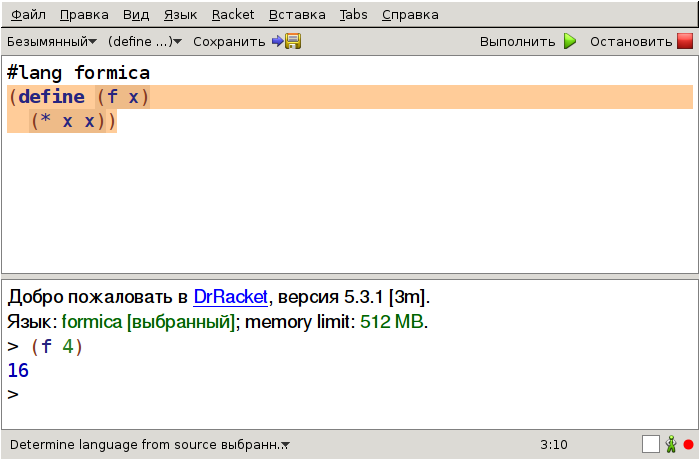
\includegraphics[width=0.9\textwidth]{../figures/DrRacket.png}}; 
   \node at (0,1) {\textsl{область определений}};
   \node at (0,-2) {\textsl{область диалога}};
   \end{tikzpicture}
\end{center}

В нижней части окна программы \Lang{DrRacket} находится окно диалога с~интерпретатором. Приглашение к~вводу выглядит, как «> ». После того, как введено выражение, оно вычисляется при~нажатии клавиши \MenuItem{Enter}, при~этом курсор должен находиться в~конце вычисляемого выражения, в~противном случае, будет просто введён символ разрыва строки.

\section{Как читать эту книжку?}%
Замечательной особенностью языков\=/интерпретаторов является возможность создавать очень короткие программы\=/вопросы и~программы\=/эксперименты, а~так же получать незамедлительный ответ интерпретатора. 

\begin{example}{%
Введём константу и~нажмём клавишу \MenuItem{Enter}. Интерпретатор вернёт результат.}
\REPL{5}{5}
\end{example}

Все разделы нашей книги сопровождаются большим числом примеров; каждый из~них может быть выполнен в~программе \Lang{DrRacket}. Участки кода, которые можно использовать в~качестве программ выделены в~тексте следующим образом:

\begin{Definition}
(define func
 ...)
\end{Definition}

Некоторые примеры представлены в~виде короткого диалога с~интерпретатором:

\REPL
  {(question ...)}
  {answer}

Все эти примеры мы рекомендуем выполнять, по~ходу чтения. При~этом стоит экспериментировать и~вносить свои изменения, придумывать свои собственные примеры.

\section{Задания и юнит-тестирование}%
В книге приводятся задания для самостоятельной работы. Чаще всего, они заключаются в~определении тех или иных функций, при~этом большинству из~них даётся краткая спецификация такого рода:

\begin{Specification}
(test 
  (func 1 2)  ==> 3
  (func 1)    ==> 42
  ...)
\end{Specification}

\noindent Первая строчка описывает тип функции, как это принято в~функциональных языках программирования. Последующие строчки дают тестовые примеры и~ожидаемые результаты. 

Спецификация позволяет понять, что должна делать программа, как она должна реагировать на~типичные и~вырожденные случаи. Скажем, в~приведённом нами примере, функция \s{func}, вызванная с~двумя аргументами: 1~и~2, должна возвращать значение 3, а~если передать ей единственный аргумент 1, результат должен быть равен~42.

Форма \sfi{test}  последовательнно сравнивает пары своих аргументов. Если они попарно одинаковы, она ничего не возвращает. В противном случае, генерируется развёрнутый отчёт об ошибке.

Спецификацию функции можно целиком скопировать или переписать в~окно определения \Lang{DrRacket} и~использовать для тестирования создаваемых программ.

Вообще, написание любой программы, не~только функциональной, должно \emph{начинаться} со~спецификации. Существует технология программирования, называемая «разработкой через тестирование». Согласно ей, тестовые примеры, должны быть написаны до~того, как будет написана сама программа. Такой подход упрощает решение задачи «с чистого листа» и~позволяет сократить работу над~ошибками. Начиная с~середины курса, читатель (студент) должен будет сам задавать спецификации создаваемых функций, перед тем, как приступать к~написанию кода. В~идеале, это должно стать его профессиональной привычкой.

